%%%%%%%%%%%%%%%%%%%%%%%%%%%%%%%%%%%%%%%%%%%%%%%%%%%%%%%%%%%%%%%%%%%%%%%%%%%%%%%%%%%%%%%%%%%%%%%%%%%%%%
% (C) 2015, by Robert Hemstedt <CC-BY-SA 3.0>                                                        %
% This work is licensed under a Creative Commons Attribution-ShareAlike 3.0 Unported License.        %
% To view a copy of this license, visit http://creativecommons.org/licenses/by-sa/3.0/.              %
%%%%%%%%%%%%%%%%%%%%%%%%%%%%%%%%%%%%%%%%%%%%%%%%%%%%%%%%%%%%%%%%%%%%%%%%%%%%%%%%%%%%%%%%%%%%%%%%%%%%%%
\documentclass[ngerman]{beamer}
\usepackage[utf8x]{inputenc}
\usepackage{amsmath}
\usepackage{amsfonts}
\usepackage{amssymb}
%\usepackage{theorem}
\usepackage{graphicx}
\usepackage{url}
\usepackage[ngerman]{babel}
\usepackage{hyperref}
\usetheme{Madrid}
%\usecolortheme{dolphin}
\usefonttheme{structurebold}
\setbeamercovered{transparent}
\setbeamertemplate{footline}[frame number]
\setbeamertemplate{caption}[numbered]
\setbeamertemplate{navigation symbols}{}%remove navigation symbols
\setbeamertemplate{bibliography item}[text] % enumerated bibliography
\newcommand{\grad}{^{\circ}}
\title{Fast Multipole Method für Potentiale in 2D}
\author{Robert Hemstedt}
\institute[Universität Bonn -- Bonn]{
\inst{}{Rheinische Friedrich Wilhelms-Universität Bonn -- Bonn \newline \newline \tiny{betreut durch die Herren Prof. Dr. Schweitzer und Prof. Dr. Klein}}}
\date[27.04.2014]{27. April 2014}

\begin{document}

\large
\begin{frame}
\titlepage
\vfill
\begin{center}

\includegraphics[scale=0.5]{by-sa.png}\\
\tiny{This work is licensed under a Creative Commons Attribution-ShareAlike 3.0 Unported License.}
\end{center}
\end{frame}

\begin{frame}
\frametitle{Gliederung}
\tableofcontents
\end{frame}

\section{Motivation}
\begin{frame}
\frametitle{Motivation}
\begin{Beispiel}
In der Ebene seien $m$ paarweise verschiedene Punkte $\{x_1,\ldots,x_m\}$ gegeben, die jeweils die Ladungen  $\{q_1,\ldots, q_m\}$ tragen. Zusätzlich seien $n$ paarweise verschiedene Punkte $\{y_1,\ldots,y_n\}$ in der Ebene gegeben, an denen die Potentiale $\Phi(y_i)$ $(i=1,\ldots,n)$ berechnet werden sollen. Der Einfachheit halber gelte $x_i\neq y_j$ für alle $i=1\ldots m, j=1,\ldots,n$.
\end{Beispiel}
\begin{alertblock}{Frage}
In welcher Zeit können alle Potentiale an den ausgewählten Punkten berechnet werden?
\end{alertblock}
\end{frame}

\section{Klassischer Ansatz}
\frame{
\frametitle{Klassischer Ansatz -- Direktes Ausrechnen}
\begin{Fakt}
Potential: $\Phi_{x_i}(y_j) = -q_i\log(||y_j-x_i||)$\cite{FastParticle}
\end{Fakt}
Also ergeben sich für alle Potentiale an den Punkten $y_j, j=1,\ldots,n$: 
\begin{equation}\nonumber
\sum_{i=1}^m {\Phi_{x_i}(y_j)} \qquad \text{für alle }j=1,\ldots,n
\end{equation}
Also insgesamt $O(mn)$ Summationen für alle Potentiale. Insbesondere $O(m^2)$, wenn $m=n$.
}

\section{Fast Multipole Method für Potentiale}
\frame{
\frametitle{$G$-Kernel}
Bezeichne: 
\begin{equation}\nonumber
G(\mathbf{y},\mathbf{x}) := -\log(||\mathbf{x}-\mathbf{y}||)\text{ und }q(\mathbf{x}_i):=q_i\text{, also }\Phi_{\mathbf{x}_i}(\mathbf{y}_j)=G(\mathbf{y}_j,\mathbf{x}_i)q(\mathbf{x}_i)
\end{equation}
Ein Trick der FMM ist es, das Problem in die Komplexe Ebene zu legen. Identifiziere: 
\begin{align*}
\mathbf{x}=(\mathbf{x}_1,\mathbf{x}_2) \quad &\Rightarrow \quad z = \mathbf{x}_1 + i\mathbf{x}_2, \\
\mathbf{y}=(\mathbf{y}_1,\mathbf{y}_2) \quad &\Rightarrow \quad z_0=\mathbf{y}_1 + i \mathbf{y}_2, \\
G(\mathbf{y},\mathbf{x}) = \Re(G(z_0,z))\text{, mit }& G (z_0,z) = -\log(z_0-z),
\end{align*}
wobei wir hier den komplexen (Hauptzweig des) Logarithmus verwenden.
}

\begin{frame}{Expansion des $G$-Kernels}
In dieser Notation berechnet man: 
\begin{equation*}\label{potential}
\sum_{i=1}^m {G(y_j,x_i)q(x_i)} \qquad \text{für alle }i=1,\ldots,n, 
\end{equation*}
und nimmt den \emph{Realanteil}. Dabei sind die Punkte $(x_i)_{i=1,\ldots,m}$, $(y_j)_{j=1,\ldots,n}$ entsprechend in die Komplexe Ebene eingebettet.\\
Die Idee der Multipolexpansion ist es nun für einen Expansionspunkt $y_c$ den Kernel zu schreiben als 
\begin{equation}
\nonumber
G(y,x) = \sum_i G_i^y(y_c,y)G_i^x(y_c,x)
\end{equation}
\begin{alertblock}

$G_i^x(y_c,x)$ ist \emph{unabhängig} von $y$, kann also wiederverwendet werden!

\end{alertblock}
\end{frame}

\begin{frame}{Expansion des $G$-Kernels}
\normalsize
\begin{alertblock}{Konvention}
Ab sofort arbeiten wir nur noch in $\mathbb{C}$.
\end{alertblock}
\begin{Lemma}
Es seien der \emph{Quellpunkt} $z_0$, der \emph{Feldpunkt} $z$ und ein \emph{Expansionspunkt} $z_c$ nahe $z$ gegeben, d.h. $|z-z_c| \ll |z_0-z_c|$. Dann gilt: 
\begin{equation}\label{multiexp}
G(z_0,z) = \sum_{k=0}^\infty {O_k(z_0-z_c)I_k(z-z_c)}.
\end{equation}
Wobei 
\begin{align*}
 \nonumber
I_k(z)&=\frac{z^k}{k!}, k\geq 0 \text{ sowie } \\ 
O_k(z)&=\frac{(k-1)!}{z^k}, k\geq 1; \text{ und } O_0(z)=-\log(z).
\end{align*}
\end{Lemma}
\end{frame}

\begin{frame}{Expansion des $G$-Kernels}
\begin{Beweis}
\[
G(z_0,z) = -\log(z_0-z) = -\left[\log(z_0-z_c) + \log \left(1-\frac{z-z_c}{z_0-z_c}\right)\right]
\]
Taylor-Expansion von \[\log(1-\xi) = -\sum_{k=1}^\infty {\frac{\xi^k}{k} }, |\xi| < 1\] liefert das gewünschte Ergebnis mit $\xi = \frac{z-z_c}{z_0-z_c}$.
\end{Beweis}
\begin{alertblock}{}
Es ist einer der Schlüsselpunkte der FMM, dass durch Gleichung \eqref{multiexp} im $G$-Kernel $z_0$ und $z$ durch $z_c$ separiert werden.
\end{alertblock}
\end{frame}

\begin{frame}{Multipolexpansion}
\small
\begin{Satz}[Multipolexpansion]
Es seien die Punkte $z_1,\ldots, z_m$ mit Ladungen $q(z_1),\ldots,q(z_m)$ gegeben. Weiterhin seien $z_0$ und $z_c$ derart, dass $|z_i-z_c| \ll |z_0-z_c|$ für alle $i=1,\ldots,m$. Dann gilt:
\begin{equation}\nonumber
\sum_{i=1}^m {G(z_0,z_i)q(z_i)} = \sum_{i=1}^m \left[\sum_{k=0}^\infty O_k(z_0-z_c)I_k(z_i-z_c)\right] q(z_i);
\end{equation}
also die \emph{Multipolexpansion}:
\begin{equation}\label{multipolexp}
\sum_{i=1}^m {G(z_0,z_i)q(z_i)} = \sum_{k=0}^\infty O_k(z_0-z_c)M_k(z_c),
\end{equation}
mit den \emph{Momenten}:
\begin{equation}\label{moments}
M_k(z_c) =  \sum_{i=1}^m I_k(z_i-z_c) q(z_i).
\end{equation}
\end{Satz}
\end{frame}

\begin{frame}{Multipolexpansion}
\begin{figure}
\def\svgwidth{0.5\textwidth}
\input{moments.pdf_tex}
\caption{Lagesituation für Multipolexpansion}
\end{figure}
\end{frame}

\begin{frame}{Momente}
\begin{block}{Der Überlegung wert}
Die Momente \[ M_k(z_c) =  \sum_{i=1}^m I_k(z_i-z_c) q(z_i) \] sind nur von den gegebenen Ladungspunkten $z_1,\ldots,z_m$ und dem Expansionspunkt $z_c$ abhängig und brauchen nicht nochmal berechnet werden, wenn $z_0$ seine Lage ändert!
Später werden die $z_c$ Zentren von Zellen eines Gitters sein, sodass die Momente $M_k(z_c)$ häufig wiederverwendet werden können. Dies ist ein \emph{Schlüsselfaktor}, warum die FMM so schnell ist!
\end{block}

\end{frame}
\begin{frame}{Fehler der Multipolexpansion}
In \eqref{multipolexp} tritt eine \emph{unendliche} Summe auf. Fehler in der Fast Multipole Method können durch die Anzahl der ausgewerteten Terme in \eqref{multipolexp} kontrolliert werden.
\begin{Satz}[Fehler der Multipolexpansion]
Für den Fehler $E_M^p$ der Multipolexpansion gilt:
\begin{align*}
E^p_M&:= \left|\sum_{i=1}^m {G(z_0,z_i)q(z_i)} - \sum_{k=0}^p O_k(z_0-z_c)M_k(z_c)\right| \\
&\leq \frac{A}{1-\frac{R}{|z_0-z_c|}}\frac{R^{p+1}}{|z_0-z_c|^{p+1}}, 
\end{align*}
wobei $R$ der Radius eines Kreises um $z_c$ mit $|z_i-z_c| < R < |z_0-z_c|$ für alle $i=1,\ldots,m$ und $A=\sum_{i=1}^m |q_i|$.
\end{Satz}
\end{frame}

\begin{frame}{Fehler der Multipolexpansion}
\footnotesize
\begin{Beweis}
\begin{align*}
E^p_M&:= \left|\sum_{k=p+1}^\infty O_k(z_0-z_c)M_k(z_c)\right| \leq \sum_{k=p+1}^\infty |O_k(z_0-z_c)||M_k(z_c)| \\
&\leq \sum_{k=p+1}^\infty |O_k(z_0-z_c)| \left|\sum_{i=1}^m I_k(z_i-z_c) q(z_i)\right| \\
&\leq \sum_{k=p+1}^\infty |O_k(z_0-z_c)| \sum_{i=1}^m |I_k(z_i-z_c)| |q(z_i)| \\
&\leq A \sum_{k=p+1}^\infty |O_k(z_0-z_c)| \frac{R^k}{k!} \leq A \sum_{k=p+1}^\infty \frac{(k-1)!}{|z_0-z_c|^k} \frac{R^k}{k!} \\
&\leq A \sum_{k=p+1}^\infty \frac{R^k}{|z_0-z_c|^k} = \frac{A}{1-\frac{R}{|z_0-z_c|}}\frac{R^{p+1}}{|z_0-z_c|^{p+1}}
\end{align*}
\end{Beweis}
\end{frame}

\begin{frame}{Fehler der Multipolexpansion}
Sei $\rho = \frac{|z_0-z_c|}{R}$. Dann lässt sich $E^p_M$ abschätzen als 
\begin{equation*}\label{rhomultipolerror}
E^p_M \leq \frac{A}{\rho-1}\left(\frac{1}{\rho}\right)^p
\end{equation*}
\begin{block}{Bemerkung}
Je größer $\rho$, desto kleiner ist die Fehlerschranke. Beobachte, dass für den Fall $\rho \geq 2 \Leftrightarrow |z_0-z_c| \geq 2 R$:
\begin{equation*}\label{halfmultipolerror}
E^p_M \leq A\left(\frac{1}{2}\right)^p.
\end{equation*}
Damit kann man für eine vorher festgelegte Genauigkeit $\varepsilon$ die Anzahl $p$ der zu evaluierenden Momente bestimmen.
\end{block}
\end{frame}

\begin{frame}{Translationsoperatoren}
Während des Algorithmus werden mehrere Expansionspunkte benötigt. Anstatt alle Momente für einen neuen Expansionspunkt $z_{c'}$ wieder neu zu berechnen, kann man die alten Momente von $z_c$ \glqq verschieben\grqq.
\begin{Satz}[Moment-to-Moment-Translation, M2M]
Es seien die Punkte $z_1,\ldots, z_m$ mit Ladungen $q(z_1),\ldots,q(z_m)$ gegeben. Weiterhin seien $z_0$, $z_c$ und $z_{c'}$ derart, dass $|z_i-z_c| \ll |z_0-z_c|$ und $|z_i-z_{c'}| \ll |z_0-z_{c'}|$ für alle $i=1,\ldots,m$. Dann gilt
\begin{equation}\label{M2Meq}
M_k(z_{c'}) = \sum_{l=0}^k I_{k-l}(z_c-z_{c'})M_l(z_c).
\end{equation}
\end{Satz}
\end{frame}

\begin{frame}{Moment-to-Moment-Translation}
\footnotesize
\begin{Beweis}
\begin{align*}
M_k(z_{c'}) &= \sum_{i=0}^m I_k(z-z_{c'})q(z_i) \\
&=  \sum_{i=0}^m I_k\left[(z-z_c) + (z_c-z_{c'})\right]q(z_i) \\
&= \sum_{i=0}^m \sum_{l=0}^k I_l(z-z_c)I_{k-l}(z_c-z_{c'}) q(z_i)\\
&= \sum_{l=0}^k I_{k-l}(z_c-z_{c'})M_l(z_c)
\end{align*}
Dabei haben wir die Binomische Formel in der dritten Gleichung verwendet.
\end{Beweis}
\begin{block}{Bemerkung}
Durch die endliche Zahl der Summanden wird keine weitere Fehlerquelle eingeführt.
\end{block}
\end{frame}

\begin{frame}{Lokale Expansion}
Statt des Expansionspunktes $z_c$ verschieben wir jetzt den Quellpunkt $z_0$:
\begin{Satz}[Lokale Expansion und Moment-to-Local-Translation]
Mit den Bedingungen der Multipolexpansion sei ein weiterer Punkt $z_L$ nahe $z_0$, d.h. $|z_0-z_L|\ll |z_L-z_c|$ gegeben. Dann gilt die folgende \emph{lokale Expansion}
\begin{equation}\label{localexp}
\sum_{i=1}^m {G(z_0,z_i)q(z_i)} = \sum_{l=0}^\infty L_l(z_L)I_l(z_0-z_L),
\end{equation}
wobei die lokalen Expansionskoeffizienten $L_l(z_L)$ durch die folgende \emph{Moment-to-Local-Expansion}(M2L) gegeben sind:
\begin{equation}\label{M2L}
L_l(z_L)=(-1)^l\sum_{k=0}^\infty O_{l+k}(z_L-z_c)M_k(z_c).
\end{equation}
\end{Satz}
\end{frame}

\begin{frame}{Lokale Expansion}
\begin{block}{Vorschau}
Sind die lokalen Expansionskoeffizienten $L_l(z_L)$ einmal berechnet worden, ist die Gleichung \eqref{localexp} 
\[\sum_{i=1}^m {G(z_0,z_i)q(z_i)} = \sum_{l=0}^\infty L_l(z_L)I_l(z_0-z_L)
\]
unabhängig von $z_c$. Wie bei der Moment-to-Moment-Translation lässt sich auch eine Local-to-Local-Translation ausdrücken. Ein weiterer Fall, wo bereits berechnete Terme wiederverwendet werden können.

Die $z_L$ werden auch wie die $z_c$ später im Algorithmus Gitterpunkte darstellen.
\end{block}
\end{frame}

\begin{frame}{Fehler der Moment-to-Local-Translation}
Auch in \eqref{M2L} tritt eine endliche Summe auf. Es gilt:
\begin{Satz}[Fehler der M2L Translation]
Für den Fehler $E_L^p$ der Moment-to-Local-Expansion gilt:
\begin{align*}
E^p_L&:= \left|\sum_{i=1}^m {G(z_0,z_i)q(z_i)} - \sum_{l=0}^p L_l(z_L)I_l(z_0-z_L)\right|\\
&=\left|\sum_{l=p+1}^\infty L_l(z_L)I_l(z_0-z_L)\right| \leq \frac{A\left[4e(p+\rho)(\rho+1)+\rho^2\right]}{\rho(\rho-1)}\left(\frac{1}{\rho}\right)^{p+1},
\end{align*}
für alle $p\geq \max\{2, \frac{2\rho}{\rho-1}\}$, wobei $e$ die Eulersche Zahl ist und $A$ und $\rho$ wie bisher definiert sind.
\end{Satz}
\end{frame}

\begin{frame}{Local-to-Local-Translation}
\normalsize
Ähnlich der Moment-to-Moment-Translation führen wir die Local-to-Local-Translation ein:
\begin{Satz}[Local-to-Local-Translation, L2L]
Es sei $z_{L'}$ ein Punkt nahe $z_L$. Dann gilt für eine lokale Expansion mit $p$ Termen:
\begin{align}
\sum_{i=1}^m {G(z_0,z_i)q(z_i)} &\approx \sum_{l=0}^p L_l(z_L)I_l(z_0-z_L) = \sum_{l=0}^p L_l(z_{L'})I_l(z_0-z_{L'}),\nonumber\\
\text{wobei } L_l(z_{L'})&=\sum_{s=0}^{p-l} I_s(z_{L'}-z_L)L_{l+s}(z_L)\label{L2Leq}
\end{align}
\end{Satz}
\begin{block}{Bemerkung}
Wie bereits bei der M2M-Translation \eqref{M2Meq} werden bei der L2L-Translation \eqref{L2Leq} nur endliche viele Terme addiert, also keine weiteren Fehler eingeführt.
\end{block}
\end{frame}

\begin{frame}{Local-to-Local-Translation}
\begin{Beweis}
\begin{align*}
\sum_{l=0}^p L_l(z_L)I_l(z_0-z_L) &= \sum_{l=0}^p L_l(z_L)I_l\left[(z_0-z_{L'}) + (z_{L'}-z_L)\right]\\
&=\sum_{0\leq s\leq l \leq p} I_s(z_0-z_{L'}) L_l(z_L)I_{l-s}(z_{L'}-z_L)\\
&=\sum_{l=0}^p \sum_{s=l}^p I_l(z_0-z_{L'}) L_s(z_L)I_{s-l}(z_{L'}-z_L) \\
&=\sum_{l=0}^p I_l(z_0-z_{L'}) \underbrace{\sum_{s=0}^{p-l}  L_{l+s}(z_L)I_{s}(z_{L'}-z_L)}_{=L_l(z_{L'})}
\end{align*}
\end{Beweis}
\end{frame}

\begin{frame}{Zwischenzusammenfassung}
Uns stehen nun folgende Werkzeuge zur Verfügung:
\small
\begin{align*}
\text{Momente: }& M_k(z_c) =  \sum_{i=1}^m I_k(z_i-z_c) q(z_i)\\
\text{Multipolexpansion: }&\sum_{i=1}^m {G(z_0,z_i)q(z_i)} \approx \sum_{k=0}^p O_k(z_0-z_c)M_k(z_c)\\
\text{M2M-Translation: }& M_k(z_c') = \sum_{l=0}^k I_{k-l}(z_c-z_c')M_l(z_c)\\
\text{M2L-Translation: }&L_l(z_L)\approx(-1)^l\sum_{k=0}^p O_{l+k}(z_L-z_c)M_k(z_c) \\
\text{Lokale Expansion: }&\sum_{i=1}^m {G(z_0,z_i)q(z_i)} \approx \sum_{l=0}^p L_l(z_L)I_l(z_0-z_L)\\
\text{L2L-Translation: }&L_l(z_{L'})=\sum_{s=0}^{p-l} I_s(z_{L'}-z_L)L_{l+s}(z_L)
\end{align*}
\end{frame}

\section{FMM-Algorithmus}
\begin{frame}{FMM-Algorithmus}
Der Fast Multipole-Algorithmus gliedert sich in mehrere Schritte:
\begin{enumerate}
\item Erstellen einer Quad-Tree-Struktur.
\item \emph{Upward pass}.
\item \emph{Downward pass}.
\item Berechnung der Potentiale.
\end{enumerate}
\end{frame}

\begin{frame}{Erstellen der Quad-Tree-Struktur}
\begin{enumerate}
\item Lege alle Punkte in ein Quadrat. Dies bildet eine \emph{Level} 0 \emph{Zelle}.
\item Zerlege das Quadrat in Level 0 in vier Zellen (Quadrate) von Level 1.
\item Lege eine Zahl $maxl$, wie viele Punkte sich maximal innerhalb einer Zelle des Quad-Trees befinden dürfen, fest.
\item Für eine Zelle von Level $l$ mache folgendes:\\
Wenn sie mehr als $maxl$ Punkte enthält, zerlege sie in vier \emph{Tochterzellen} von Level $l+1$. Sie ist jetzt eine \emph{Vaterzelle}.\\
Sonst bildet sie ein \emph{Blatt} des Quad-Trees und wird nicht weiter zerlegt.
\item Fahre mit obigem Schritt fort, bis keine Zelle mehr in Quadrate zerlegt wird.
\end{enumerate}
\end{frame}

\begin{frame}{Erstellen der Quad-Tree-Struktur}
\begin{figure}
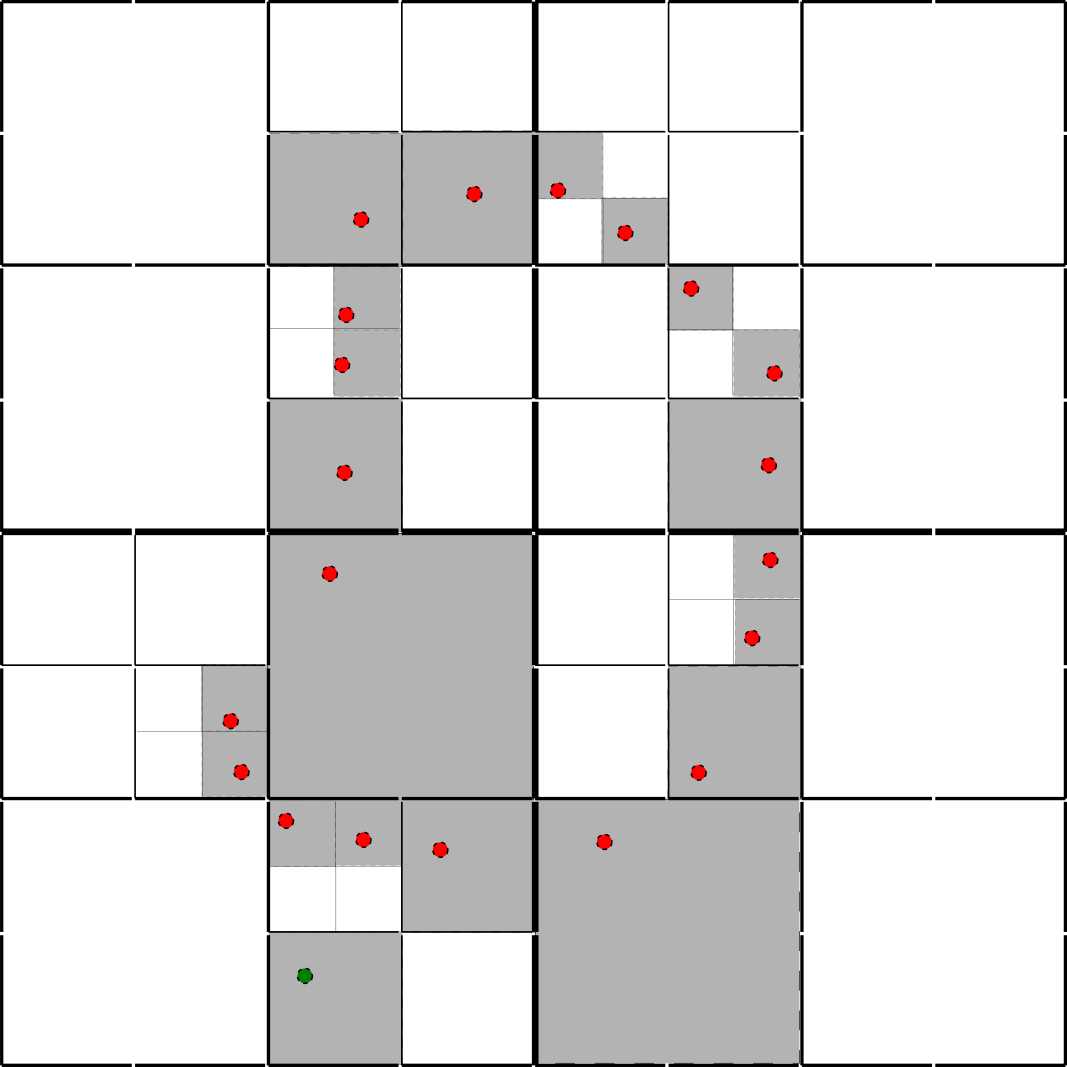
\includegraphics[width=0.5\textwidth]{quadtree.png}
\caption{Quad-Tree der geladenen Punkte (rot), eines Quellpunktes (grün) und Blätter (grau)}
\end{figure}
\end{frame}

\begin{frame}{Upward pass}
Berechnung aller Momente aller Zellenzentren von Level $\geq 2$ mit $p$ Termen, beginnend bei den Blättern:
\begin{itemize}
\item Handelt es sich bei der Zelle um ein Blatt, berechne das Moment der Zelle mittels der Gleichung \eqref{moments} für alle geladenen Punkte innerhalb des Blattes, dabei ist $z_c$ das Zentrum der Zelle.
\item Handelt es sich um eine Vaterzelle, berechne ihr Moment mittels der Summation der M2M-Translationen \eqref{M2Meq} der Zentren ihrer Tochterzellen, dabei ist $z_{c'}$ das Zentrum der Vaterzelle und $z_c$ das Zentrum einer Tochterzelle.
\end{itemize}
\end{frame}

\begin{frame}{Upward pass}
\begin{figure}
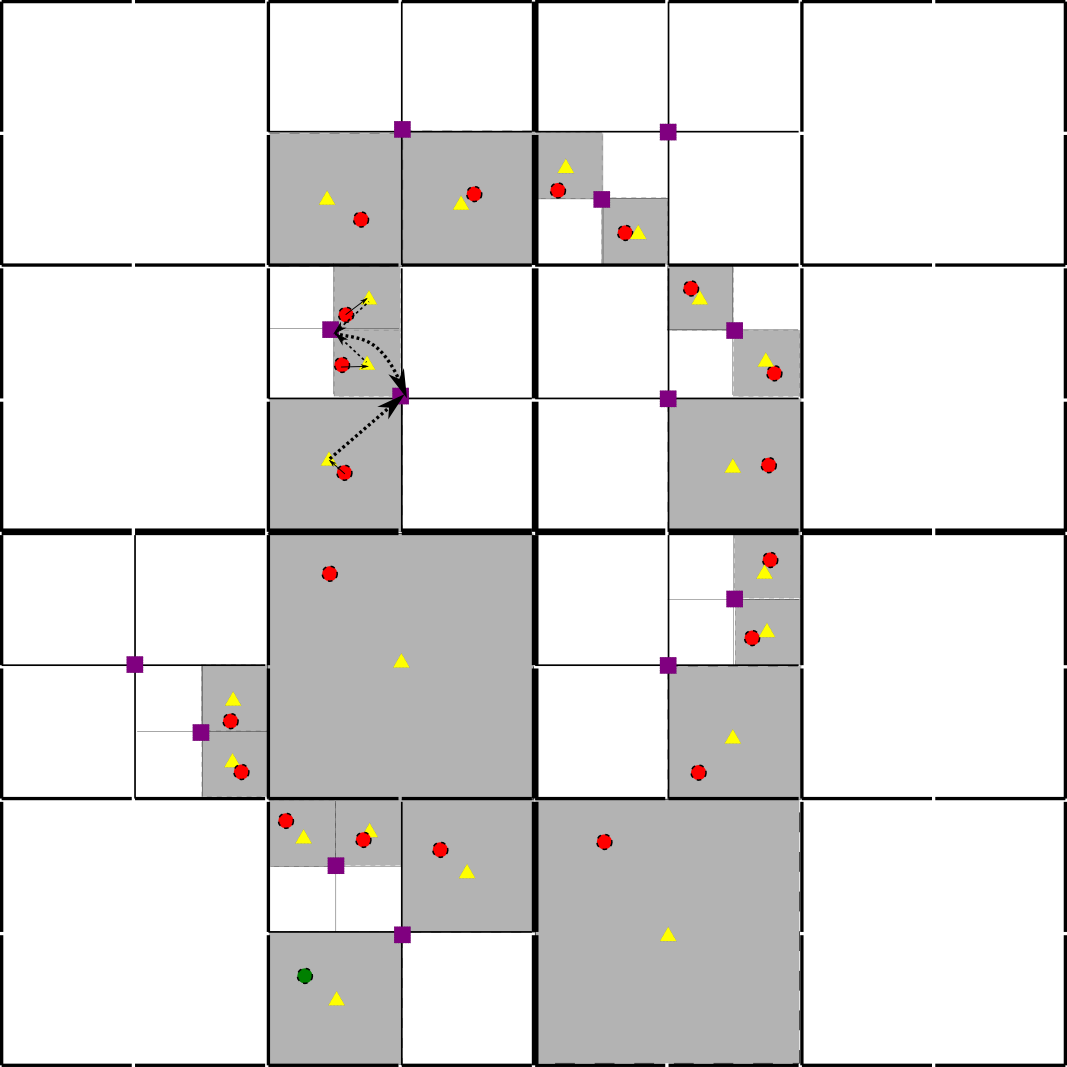
\includegraphics[width=0.5\textwidth]{upward.png}
\caption{Beispielhafter Upward pass von einer Blattzelle. \linebreak violett: Zentren von Vaterzellen, gelb: Zentren von Blättern,\linebreak $\rightarrow$: Moment direkt berechnet, $\dashrightarrow$: M2M-Translation}
\end{figure}
\framezoom<1><2>[border](4cm,1.5cm)(2cm,2cm)
\end{frame}

\begin{frame}{Downward pass}
Hierfür benötigen wir noch etwas mehr Vokabular:
\begin{Definition}
\begin{itemize}
\item Zwei Zellen heißen \emph{benachbart in Level $l$}, wenn sie mindestens eine gemeinsame Ecke haben. Zwei Blattzellen verschiedener Level sind dann benachbart, falls die Vaterzelle einer Zelle mit der anderen Zelle mindestens eine Ecke gemeinsam hat.
\item Zwei Zellen heißen \emph{gut separiert in Level $l$}, wenn sie auf Level $l$ \emph{nicht benachbart sind}, aber ihre \emph{Vaterzellen in Level $l-1$ benachbart} sind.
\item Bezeichne die Menge aller gut separierten Zellen einer Zelle $C$ in Level $l$ als \emph{Interaktionsliste} von $C$.
\item Eine Zelle ist eine \emph{Fernzelle} von $C$, wenn ihre jeweiligen Vaterzellen nicht benachbart sind.
\end{itemize}
\end{Definition}
\end{frame}

\begin{frame}{Downward pass}
\begin{figure}
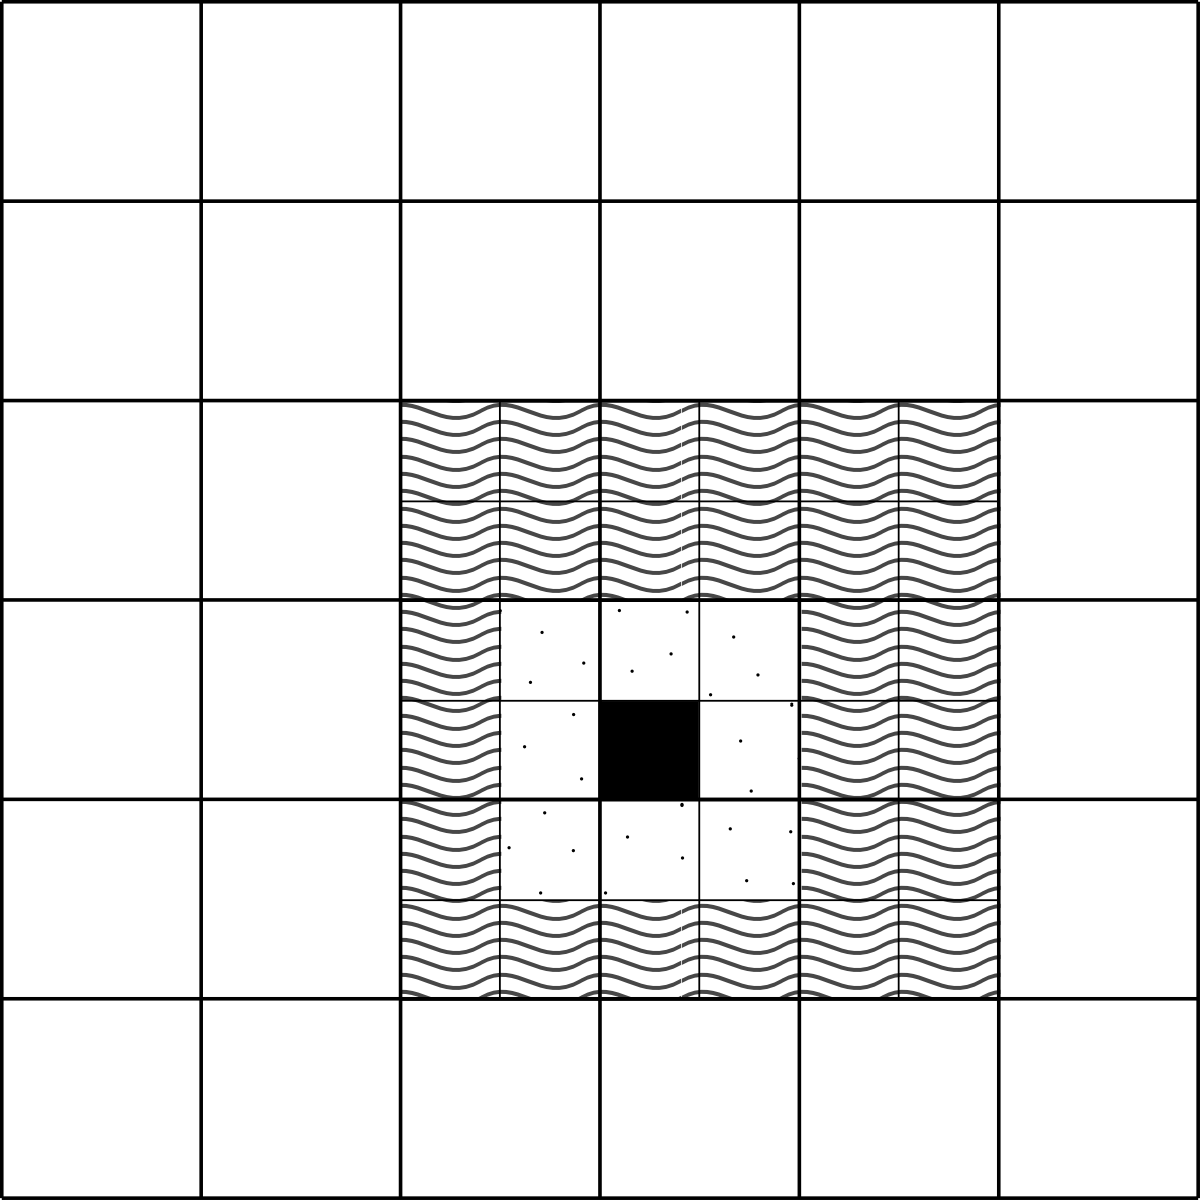
\includegraphics[width=0.5\textwidth]{intlist.png}
\caption{schwarz: Zelle $C$, gepunktet: ihre benachbarten Zellen, \linebreak gewellt: ihre Interaktionsliste, weiß: Fernzellen von $C$}
\end{figure}
\end{frame}

\begin{frame}{Downward pass}
Berechnung aller lokalen Expansionskoeffizienten aller Zellen startend bei Level $2$ und die Baumstruktur nach unten zu allen Blättern folgend.\\
\begin{enumerate}
\item\label{locexpsum} Der lokale Expansionskoeffizient einer Zelle $C$ ist die Summe 
\begin{enumerate} 
\item\label{intlist} der Beiträge der Zellen von der Interaktionsliste von $C$ und 
\item\label{farcell} von allen Fernzellen.
\end{enumerate}
\item \ref{locexpsum}.\ref{intlist} benutzt M2L-Translation \eqref{M2L}, wobei die Momente die der Zellen der Interaktionsliste sind.
\item \ref{locexpsum}.\ref{farcell} benutzt L2L-Translation \eqref{L2Leq} um den lokalen Expansionspunkt vom Zentrum der Vaterzelle von $C$ zum Zentrum von $C$ zu verschieben.
\item Auf Level 2 wird für den lokalen Expansionskoeffizienten M2L-Translation verwendet. Dabei werden die Beiträge der in Level 2 nicht benachbarten Zellen aufsummiert. 
\end{enumerate}
\end{frame}

\begin{frame}{Downward pass}
\begin{figure}
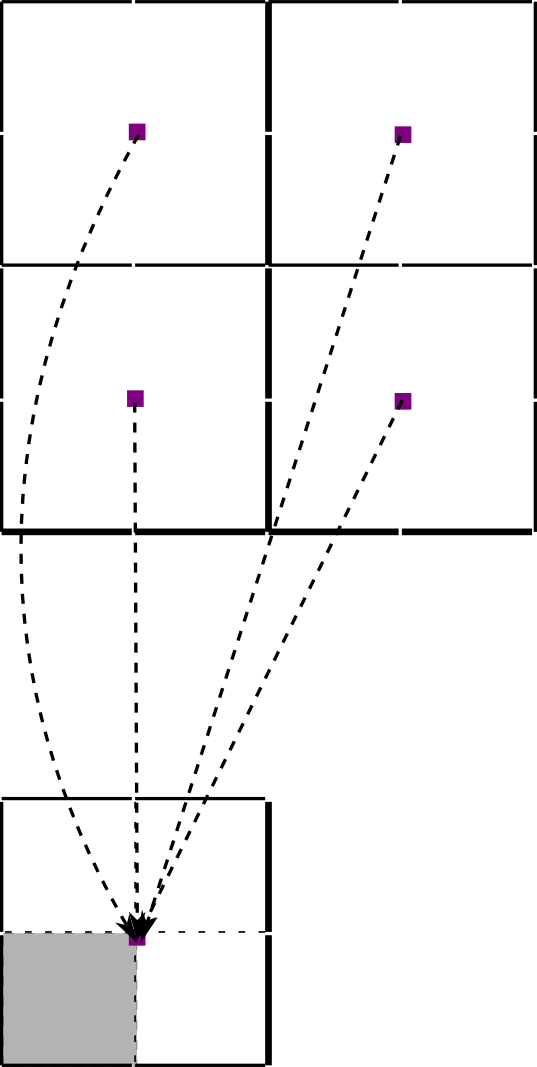
\includegraphics[height=0.5\textwidth]{downpass1.png}
\caption{Downward Pass bei Level 2. $\dashrightarrow$: M2L-Translation}
\end{figure}
\end{frame}

\begin{frame}{Downward pass}
\begin{figure}
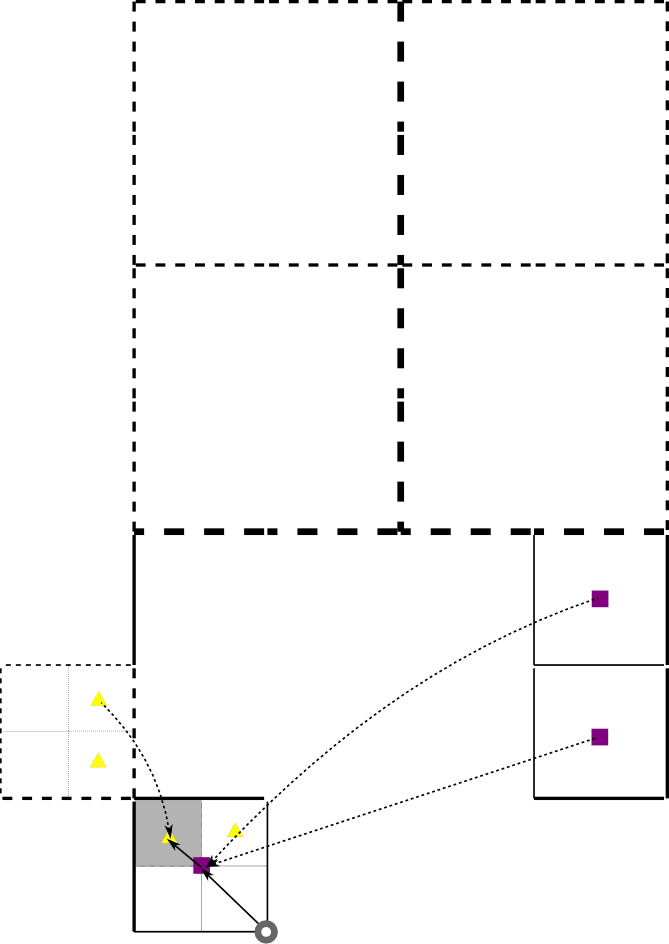
\includegraphics[height=0.5\textwidth]{downpass2.png}
\caption{Downward Pass bei Leveln 3 und 4. $\dashrightarrow$: M2L-Translation, $\rightarrow$: L2L-Translation, Kreis: Zellzentrum Level 2, Quadrat: Zellzentrum Level 3, Dreieck: Zellzentrum Level 4}
\end{figure}
\framezoom<1><2>[border](3.5cm,3.5cm)(5cm,3cm)
\end{frame}

\begin{frame}{Berechnung der Potentiale}
Für die Punkte an denen das Potential berechnet werden soll, erfolgt nun die Berechnung dessen.\\
Sei $z_0$ in Blatt $C$.
Dann berechnen wir 
\begin{align*}
\Phi(z_0) &= \Phi_{\text{nah}}(z_0) + \Phi_{\text{fern}}(z_0) &\\
\sum_{i=1}^m {G(z_0,z_i)q(z_i)} &= \underbrace{\sum_{z_i\text{ nahe } z_0 } G(z_0,z_i)q(z_i)}_{\text{Nahwirkung}} + \underbrace{\sum_{z_i\text{ fern }z_0} G(z_0,z_i)q(z_i)}_\text{Fernwirkung},
\end{align*}
wobei wir für die $z_i$, die sich in $C$ oder einen seiner acht Nachbarzellen befinden, die \emph{Nahwirkung} mit \emph{direkter} Summation auswerten. Hingegen verwenden wir für die Fernwirkung, also Beiträge aus der Interaktionsliste von $C$ und fernen Zellen, die Lokalexpansion der Zelle $C$, also \eqref{localexp}, wobei $z_L$ das Zentrum von $C$ ist.
\end{frame}

\begin{frame}{Laufzeitanalyse}
Zurück zur am Anfang gestellten Frage. Sind wir mit dem FMM-Algorithmus wirklich schneller?
\begin{Satz}[Laufzeit des FMM-Algorithmus]
Sei $N$ die Anzahl der geladenen Teilchen und $N$ die Anzahl der Punkte deren Potentiale, verursacht durch die geladenen Teilchen, berechnet werden sollen. Sei $p$ die Anzahl der Terme die für die Multipol- und Lokalexpansionen verwendet werden und $maxl$ die maximale Anzahl von geladenen Teilchen in einem Blatt des Quad-Trees. Dann ist die Berechnung aller Potentiale mit dem hier vorgestellten Fast-Multipole-Method-Algorithmus in Laufzeit $\mathcal{O}(N)$ möglich.
\end{Satz}
\end{frame}

\begin{frame}{Laufzeitanalyse}
\begin{Beweis}
\footnotesize
\begin{itemize}
\item $N_\text{B}$ = Anzahl der Blätter im Quad-Tree $\approx N/maxl = \mathcal{O}(N)$
\item $N_\text{Z}$ = Anzahl der Zellen im Quad-Tree $\approx N_\text{B}\cdot(1+\frac{1}{4} + \frac{1}{4^2} + \ldots) \leq N_\text{B} \cdot \frac{4}{3} = \mathcal{O}(N)$
\item Anzahl benachbarter Zellen = 9; Anzahl der Zellen in der Interaktionsliste = 27 (2D)
\item Anzahl Operationen, um Multipolmomente zu berechnen = $p\cdot maxl \cdot N_\text{B} = \mathcal{O}(N)$
\item Anzahl Operationen im Upward pass = $N_\text{Z}\cdot 4 \cdot p^2 = \mathcal{O}(N)$
\item Anzahl Operationen im Downward pass = $N_\text{Z}\cdot \left[p^2 (L2L) + 27 \cdot p^2(M2L) \right] = \mathcal{O}(N)$
\item Anzahl Operationen der Lokalexpansionen = $N \cdot p = \mathcal{O}(N)$
\item Anzahl Operationen der direkten Berechnungen der Potentiale der Nahwirkung = $N\cdot 9\cdot maxl = \mathcal{O}(N)$
\end{itemize}
Alle Abschätzungen haben höchstens Laufzeit $\mathcal{O}(N)$, damit ist die Gesamtlaufzeit $\mathcal{O}(N)$.
\end{Beweis}
\end{frame}

\begin{frame}{Literaturverzeichnis}
\nocite{*}
\bibliographystyle{plain}
\bibliography{sources}
\end{frame}

\end{document}